% Figure 4: directional effects of depth-wise score corrections (image2.svg).
\begin{figure*}[t]
\centering
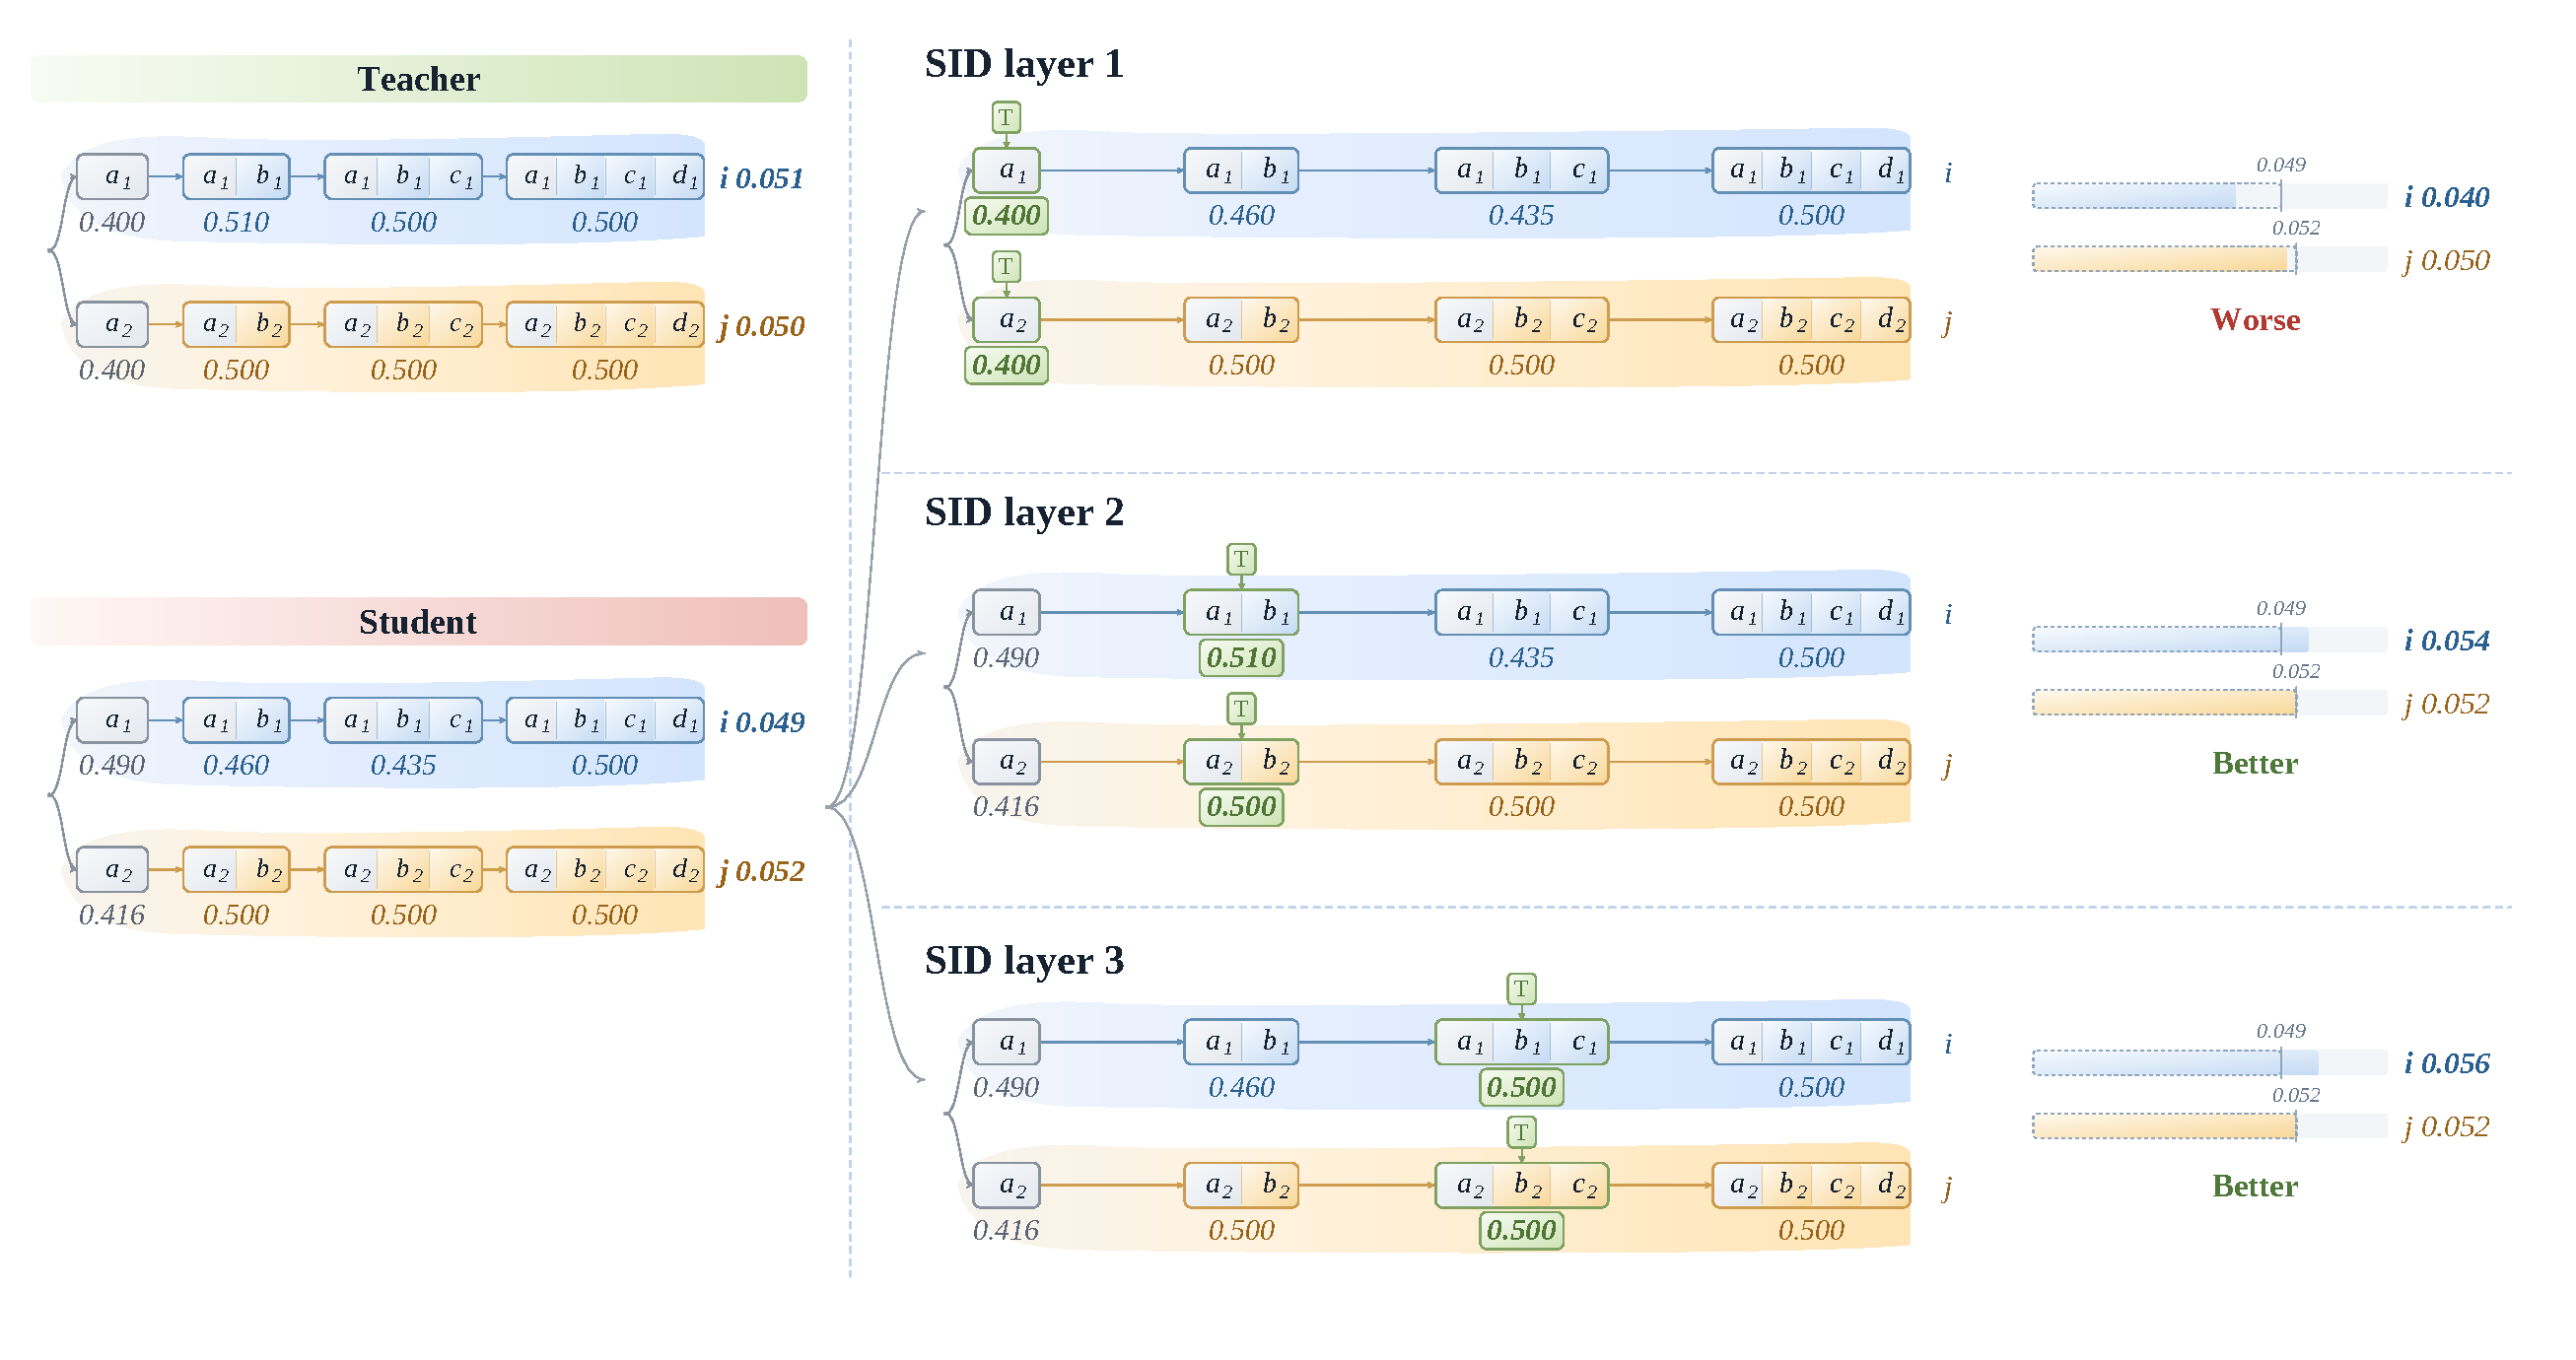
\includegraphics[width=0.945\textwidth]{Figures/diag_replace.pdf}
\caption{Illustrative single-depth replacement of a student's
local log-probability increments by teacher increments, keeping the
other depths fixed. Item scores sum the local increments; a check
indicates recovery of the teacher-preferred pairwise order, not a
measured NDCG gain or a training update.}
\Description{A candidate-pair schematic compares three single-SID-depth
replacements. A check means the teacher-preferred pairwise order
is restored; a cross means the order remains reversed.}
\label{fig:ranking_depth}
\end{figure*}
